% Assignment 01 submission source.
% Replace the two identity macros below before final submission.
% All report content and diagram semantics are condensed from
% storage/data/A01_Fashion_ECommerce_Information_System_Investigation.md.
\documentclass[10pt,a4paper]{article}

\usepackage[a4paper,top=14mm,bottom=14mm,left=14mm,right=14mm,headsep=3mm,footskip=7mm]{geometry}
\usepackage{microtype}
\usepackage[table]{xcolor}
\usepackage{booktabs,tabularx,array,multirow}
\usepackage{enumitem}
\usepackage{titlesec}
\usepackage{graphicx}
\graphicspath{{../img/}}
\usepackage{tikz}
\usetikzlibrary{arrows.meta,backgrounds,calc,fit,matrix,positioning,shapes.geometric}
\usepackage{multicol}
\usepackage{float}
\usepackage{caption}
\usepackage[hidelinks]{hyperref}
\usepackage{ragged2e}
% ---------- Identity (replace before submission) ----------
\newcommand{\studentid}{[Insert Student ID]}
\newcommand{\studentname}{[Insert Student Name]}
\hypersetup{
  pdftitle={ABC Fashion Online Shop -- E-Commerce Information System Investigation},
  pdfsubject={Information System Analysis and Design -- Assignment 01},
  pdfauthor={\studentname}
}

% ---------- Restrained academic palette ----------
% Body text is black; pale blue is reserved for diagram emphasis only.
\definecolor{Ink}{HTML}{111111}
\definecolor{RuleGray}{HTML}{666666}
\definecolor{TableGray}{HTML}{EDEDED}
\definecolor{LaneGray}{HTML}{F7F7F7}
\definecolor{DiagramBlue}{HTML}{DCEEF5}
\color{Ink}
\setlength{\parindent}{0pt}
\setlength{\parskip}{2.1pt}
\setlength{\emergencystretch}{1.5em}
\setlength{\tabcolsep}{2.8pt}
\renewcommand{\arraystretch}{1.13}
\setlist[itemize]{leftmargin=3.8mm,itemsep=0.4pt,topsep=1pt,parsep=0pt}
\setlist[enumerate]{leftmargin=4.5mm,itemsep=0.4pt,topsep=1pt,parsep=0pt}
\titleformat{\section}{\normalfont\Large\bfseries}{\thesection.}{.5em}{}
\titleformat{\subsection}{\normalfont\normalsize\bfseries}{\thesubsection.}{.45em}{}
\titlespacing*{\section}{0pt}{4pt}{2pt}
\titlespacing*{\subsection}{0pt}{3pt}{1pt}
\captionsetup{font=footnotesize,labelfont=bf,skip=2pt}
\pagestyle{plain}

\newcolumntype{Y}{>{\RaggedRight\arraybackslash}X}
\newcolumntype{L}[1]{>{\RaggedRight\arraybackslash}p{#1}}
\newcommand{\tighttable}{\fontsize{7.15}{8.1}\selectfont}
\newcommand{\tinytab}{\fontsize{6.65}{7.4}\selectfont}
\newcommand{\keyterm}[1]{\textbf{#1}}

% Figure styles. These preserve the native visual grammar expected in
% Visual Paradigm: mind-map hierarchy, BPMN events/tasks/gateways/pools,
% Yourdon-style context DFD entities/process/flows, and causal tree arrows.
\tikzset{
  vpRoot/.style={ellipse,draw=Ink,thick,fill=DiagramBlue,text=Ink,
    font=\bfseries\sffamily\scriptsize,align=center,inner sep=4pt},
  vpInternal/.style={rectangle,draw=Ink,thick,fill=TableGray,
    font=\bfseries\sffamily\scriptsize,align=center,inner sep=3pt},
  vpExternal/.style={rectangle,draw=Ink,thick,fill=TableGray,
    font=\bfseries\sffamily\scriptsize,align=center,inner sep=3pt},
  vpLeaf/.style={rectangle,draw=Ink,fill=white,
    font=\sffamily\scriptsize,align=center,inner sep=2.5pt},
  mmLine/.style={draw=Ink,semithick},
  bpmnTask/.style={rounded corners=2.4pt,draw=Ink,thick,fill=DiagramBlue,
    minimum height=7mm,text width=22mm,align=center,font=\sffamily\scriptsize,inner sep=1.4pt},
  bpmnHuman/.style={bpmnTask,fill=white,draw=Ink},
  bpmnGateway/.style={diamond,aspect=1.35,draw=Ink,thick,fill=white,
    minimum size=8mm,align=center,font=\sffamily\scriptsize,inner sep=.2pt},
  bpmnEvent/.style={circle,draw=Ink,thick,fill=white,minimum size=4.6mm,inner sep=0pt},
  bpmnEnd/.style={bpmnEvent,double,double distance=.7pt},
  sequence/.style={-{Stealth[length=2mm]},draw=Ink,thick},
  message/.style={-{Stealth[open,length=2mm]},draw=RuleGray,thick,dashed},
  pool/.style={draw=Ink,thick,fill=white},
  lane/.style={draw=RuleGray,thin},
  dfdEntity/.style={rectangle,draw=Ink,thick,fill=white,
    text width=28mm,minimum height=8mm,align=center,font=\sffamily\scriptsize,inner sep=1.6pt},
  dfdProcess/.style={circle,draw=Ink,thick,fill=DiagramBlue,
    text width=35mm,minimum height=22mm,align=center,font=\bfseries\sffamily\scriptsize},
  dataflow/.style={-{Stealth[length=1.8mm]},draw=Ink,semithick},
  flowlabel/.style={font=\sffamily\fontsize{6.1}{6.5}\selectfont,fill=white,inner sep=.6pt,align=center},
  cause/.style={rectangle,draw=Ink,thick,fill=white,
    text width=35mm,minimum height=10mm,align=center,font=\sffamily\scriptsize},
  focal/.style={ellipse,draw=Ink,thick,fill=DiagramBlue,
    text=Ink,text width=54mm,minimum height=12mm,align=center,font=\bfseries\sffamily\footnotesize},
  effect/.style={rectangle,draw=Ink,thick,fill=TableGray,
    text width=35mm,minimum height=10mm,align=center,font=\sffamily\scriptsize},
  causal/.style={-{Stealth[length=2mm]},draw=Ink,semithick}
}

\begin{document}

% ============================== PAGE 1 ==============================
\hypersetup{pageanchor=false}
\begin{titlepage}
\thispagestyle{empty}
\vspace*{5mm}
\noindent\colorbox{TableGray}{%
\begin{minipage}[c][57mm][c]{0.16\textwidth}
  \centering
  
\includegraphics[width=24mm]{logo.png}
\end{minipage}%
\begin{minipage}[c][57mm][c]{0.64\textwidth}
  \centering
  {\large\textsc{Posts and Telecommunications Institute of Technology}\par}
  \vspace{2mm}
  {\LARGE\bfseries Assignment 01\par}
  \vspace{1.5mm}
  {\large E-Commerce Information System Investigation\par}
  \vspace{2mm}
  \textbf{Information System Analysis and Design}
  \vspace{2mm}

  \begin{multicols}{2}
  \raggedright\small
  \textbf{Student:} \studentname\\
  \textbf{Student ID:} \studentid

  \columnbreak
  \textbf{Domain:} Fashion E-Commerce\\
  \textbf{Date:} 26 August 2026
  \end{multicols}
\end{minipage}%
\begin{minipage}[c][57mm][c]{0.16\textwidth}
  \centering
  {\Huge\bfseries A01\par}
  \vspace{2mm}
  {\small ABC Fashion\\Online Shop\par}
\end{minipage}}

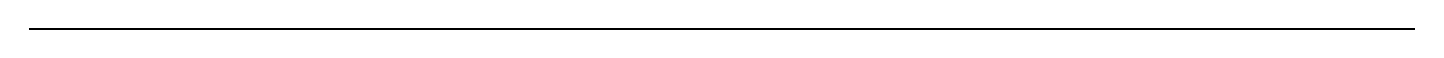
\begin{tikzpicture}
  \draw[thick] (0,0)--(17.6,0);
\end{tikzpicture}

\section*{Executive Summary}
ABC Fashion Online Shop is modeled as a medium-sized B2C retailer that owns and sells apparel, footwear, and accessories online. The investigation identifies one focal problem: fragmented and unreliable information prevents the business from coordinating Product Variants, stock, Orders, payment results, delivery, returns, customers, and reporting as one end-to-end process. In fashion, the stocked and fulfilled unit is the exact size/color \keyterm{Product Variant}, not its parent Product Style.

The proposed \keyterm{ABC Fashion Commerce Information System (AFCIS)} establishes a controlled information backbone for catalog, customer, cart, Order, promotion, variant-level inventory, fulfillment, after-sales, review, and operational reporting. Payment execution, carrier operations, and message delivery remain external services. Six problems are established by the assignment case; return/exchange and promotion-control concerns remain hypotheses for validation before Assignment 02.

\vfill
\begin{center}
\small Required submission filename: \texttt{A01\_StudentID\_Name.pdf}
\end{center}
\end{titlepage}
\hypersetup{pageanchor=true}

% ============================== PAGE 2 ==============================
\section{Introduction}
This report answers the assignment's central question: \emph{What problem should the information system solve?} It follows the required progression from organization and activities through stakeholders, information, problems, scope, boundary, and objectives. It is a desk-based investigation grounded in the Assignment 01 case and the completed fashion-domain analysis; detailed UML, database, interface, and implementation design are intentionally deferred.

\textbf{Assumptions and limits.} ABC is treated as one medium-sized, owned-inventory B2C retailer with one initial warehouse and an online storefront. Payment authorization, physical transport, and message delivery are performed by external providers. The case supplies no interviews, logs, policies, or measured baselines; therefore, fashion-specific failure modes and numeric targets are explicitly preliminary.

\textbf{Controlled terms.} A \keyterm{Product Style} groups related merchandise; a \keyterm{Product Variant} is one sellable size/\allowbreak color/\allowbreak attribute combination with one SKU. It is the stock, order-line, fulfillment, return, and exchange unit. \keyterm{Available-to-\allowbreak Sell (ATS)} is eligible on-hand stock less reservations and approved safety stock.

\section{Business Background}
\subsection{Organization}
ABC Fashion Online Shop selects, purchases, markets, sells, fulfills, and supports its own assortment of apparel, footwear, and accessories through online channels. Its purpose is to convert a managed assortment into reliable orders while supplying enough size, fit, color, price, availability, delivery, and return information for confident customer decisions.

\subsection{Business Model}
\begin{tabularx}{\textwidth}{L{30mm}Y}
\rowcolor{TableGray}\textbf{Aspect} & \textbf{Investigation finding}\\
Customer/value & Online consumers; convenient discovery, trustworthy variant availability, and transparent order/after-sales status.\\
Revenue/channel & Owned-merchandise sales through a responsive online storefront, net of promotions, returns, refunds, and fulfillment costs.\\
Relationships & Self-service browsing, cart, checkout, tracking, reviews, returns/exchanges, and staff-assisted support.\\
Resources and partners & Product and stock information, staff, warehouse, suppliers, Payment Gateway, Shipping Provider, and Notification Service.\\
\end{tabularx}

\subsection{Products and Customers}
The assortment covers apparel, footwear, and accessories. Customers need search and filtering by category, price, size, color, material, fit, and availability; variant-consistent media and size guidance; accurate promotion and ATS information; and dependable payment, shipment, return, exchange, and refund status. A style can be browsed as one family, but selection must resolve to a unique SKU before checkout.

\subsection{Major Business Activities}
ABC manages assortment and variants; prices/promotions; customers and consent; browsing/search; cart/checkout; orders and payments; variant-level stock; picking, packing, shipping and tracking; customer service, cancellations, returns/exchanges/refunds; reviews; supplier receipts; and sales/stock/operations reporting.

\textbf{Business objectives:} trustworthy product presentation; fulfillment of the exact promised variant; less re-keying and disconnected handoffs; timely self-service status and after-sales support; and timely, reconcilable management information.

\vfill
\colorbox{TableGray}{\parbox{\dimexpr\textwidth-2\fboxsep}{\footnotesize
\textbf{Evidence discipline.} Inconsistent products, outdated inventory, manual order work, unclear order status, fragmented customer records, manual reports, and limited real-time information are case facts. Specific variant, returns, and promotion failure modes are hypotheses until validated.}}
\newpage

% ============================== PAGE 3 ==============================
\section{Stakeholder Analysis}
Internal/external classification is relative to ABC as an organization. Employees later appear as external entities in the context DFD because they stand outside the AFCIS software boundary.

\subsection{Internal Stakeholders}
Owner/General Manager; E-Commerce Administrator; Merchandiser/Catalog Staff; Marketing/Promotion Staff; Sales and Customer Service Staff; Warehouse/Fulfillment Staff; and Finance/Accounting Staff.

\subsection{External Stakeholders}
Customer; Supplier; Payment Gateway; Shipping Provider; and Notification Service.

\subsection{Stakeholder Interests}
\begin{tabularx}{\textwidth}{L{30mm}L{38mm}Y L{23mm}}
\rowcolor{TableGray}\textbf{Stakeholder} & \textbf{Role} & \textbf{Main interest / need} & \textbf{Influence}\\
Owner / Manager & Sponsor and policy owner & Benefits, risks, reliable KPIs and timely exceptions & High\\
Administrator & Access, settings, exceptions & Efficient, accurate and auditable control & High\\
Merchandiser / Marketing & Catalog and promotions & One controlled variant source and deterministic rules & High\\
Sales / Customer Service & Order and after-sales support & Consolidated customer/order lifecycle status & High\\
Warehouse / Fulfillment & Stock and physical events & Exact-SKU work, accurate balances and traceability & High\\
Finance / Accounting & Reconciliation & Linked order, payment, refund and fee information & Med--high\\
Customer & Browse, buy, track, return, review & Confidence, accurate availability, fair price and status & High interest\\
Supplier & Provide merchandise/facts & Clear receipt and replenishment communication & Medium\\
Payment / Shipping providers & Financial and delivery services & Valid requests, stable references and exception handling & High interface\\
Notification Service & Message delivery & Valid destination/content and correlation reference & Medium\\
\end{tabularx}

\begin{figure}[H]
\centering
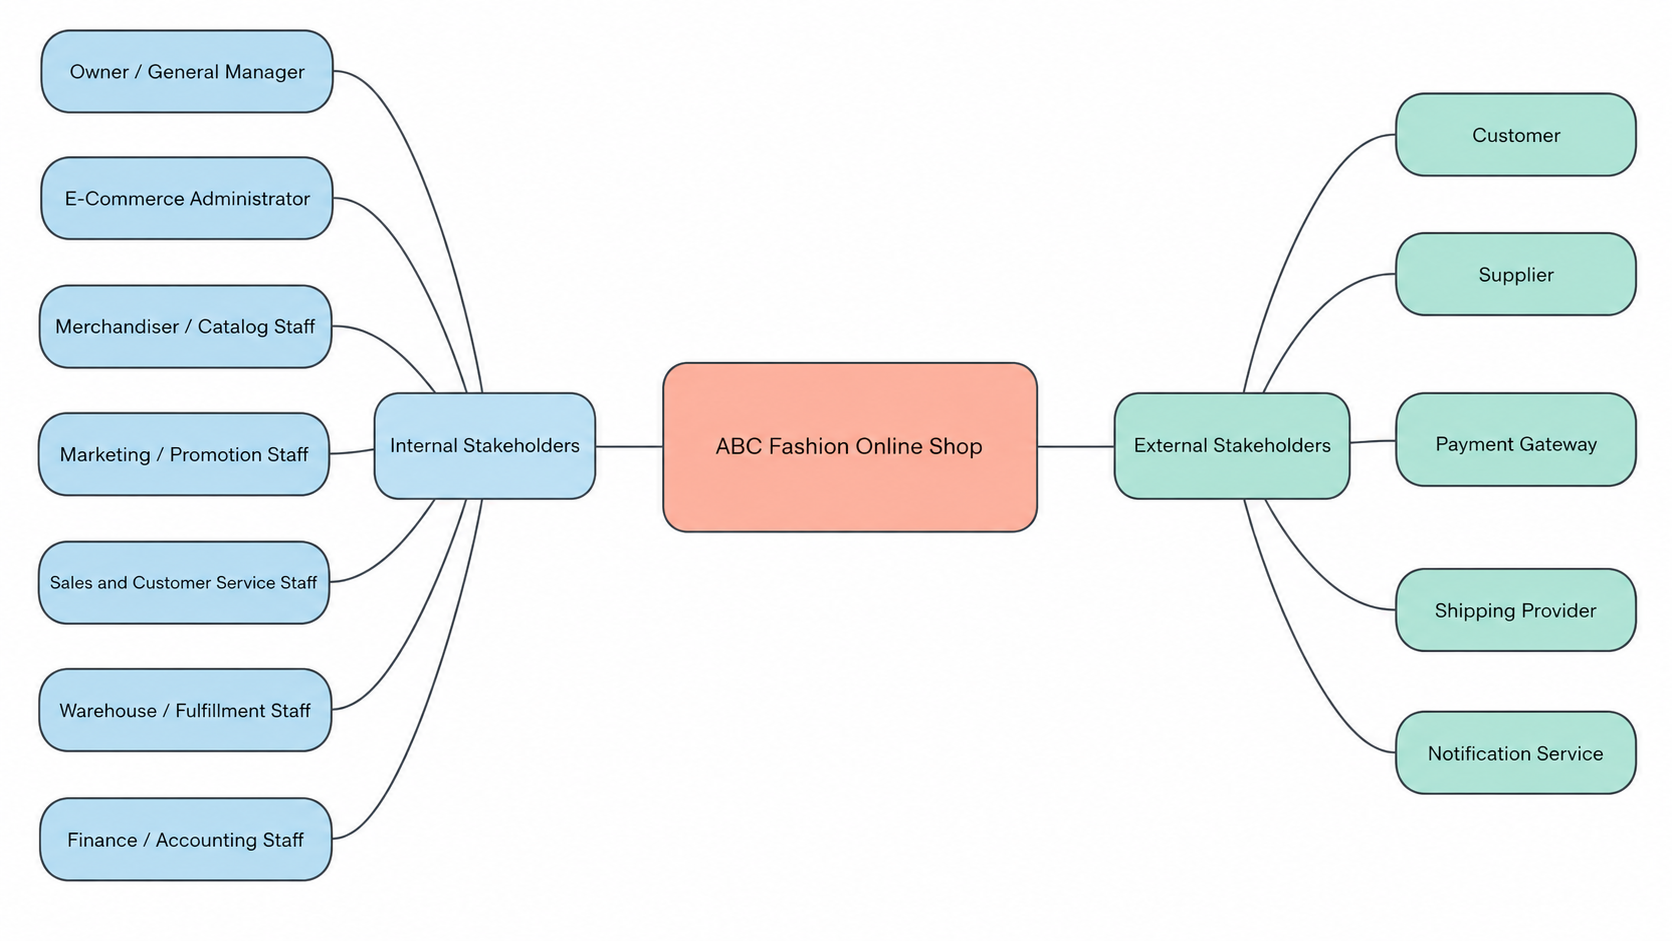
\includegraphics[width=0.98\textwidth]{stakeholder_map.png}
\caption{Core Diagram 1 --- Stakeholder Map for ABC Fashion Online Shop.}
\label{fig:stakeholder-map}
\end{figure}

The map contains all and only the stakeholder groups analyzed above. Branch connectors indicate classification, not authorization or data flow; therefore, UML actors and Use Cases are not used.
\newpage

% ============================== PAGE 4 ==============================
\section{Business Activity Analysis}
\begin{tabularx}{\textwidth}{L{29mm}Y L{43mm}}
\rowcolor{TableGray}\textbf{Required activity} & \textbf{Role in the business} & \textbf{Principal information}\\
\textbf{4.1 Product Management} & Maintains categories, Styles, Variants, images, size/fit/care, lifecycle, prices and publication. & Style/Variant, media, price, promotion, supplier facts\\
\textbf{4.2 Customer Management} & Maintains one controlled identity, contact, address, consent and service timeline. & Customer, consent, address, service history\\
\textbf{4.3 Order Processing} & Validates cart, price, promotion and ATS; snapshots exact SKU lines; reserves stock and controls status. & Cart, Order, Order Line, reservation, status event\\
\textbf{4.4 Payment} & Sends authorization/capture/refund requests to the gateway and records results/references. & Amount, request, gateway reference/status; no raw PAN/CVV\\
\textbf{4.5 Inventory} & Records SKU/location receipts, reservations, releases, picks, shipments, returns and adjustments. & On-hand, reserved, ATS, movement and source reference\\
\textbf{4.6 Shipping} & Directs exact-SKU pick/pack, requests shipment, and maps tracking milestones into lifecycle status. & Pick list, package, address, tracking/status\\
\textbf{4.7 Reporting} & Produces defined sales, stock, fulfillment, return/refund, promotion and exception views. & Governed operational data, period/status filters, refresh time\\
\end{tabularx}

Browsing and fit support, cart and checkout, promotions, reviews, cancellation, return, exchange, refund, and supplier receipt complete the required fashion journey.

\iffalse
\begin{figure}[!h]
\centering
\resizebox{\textwidth}{!}{%
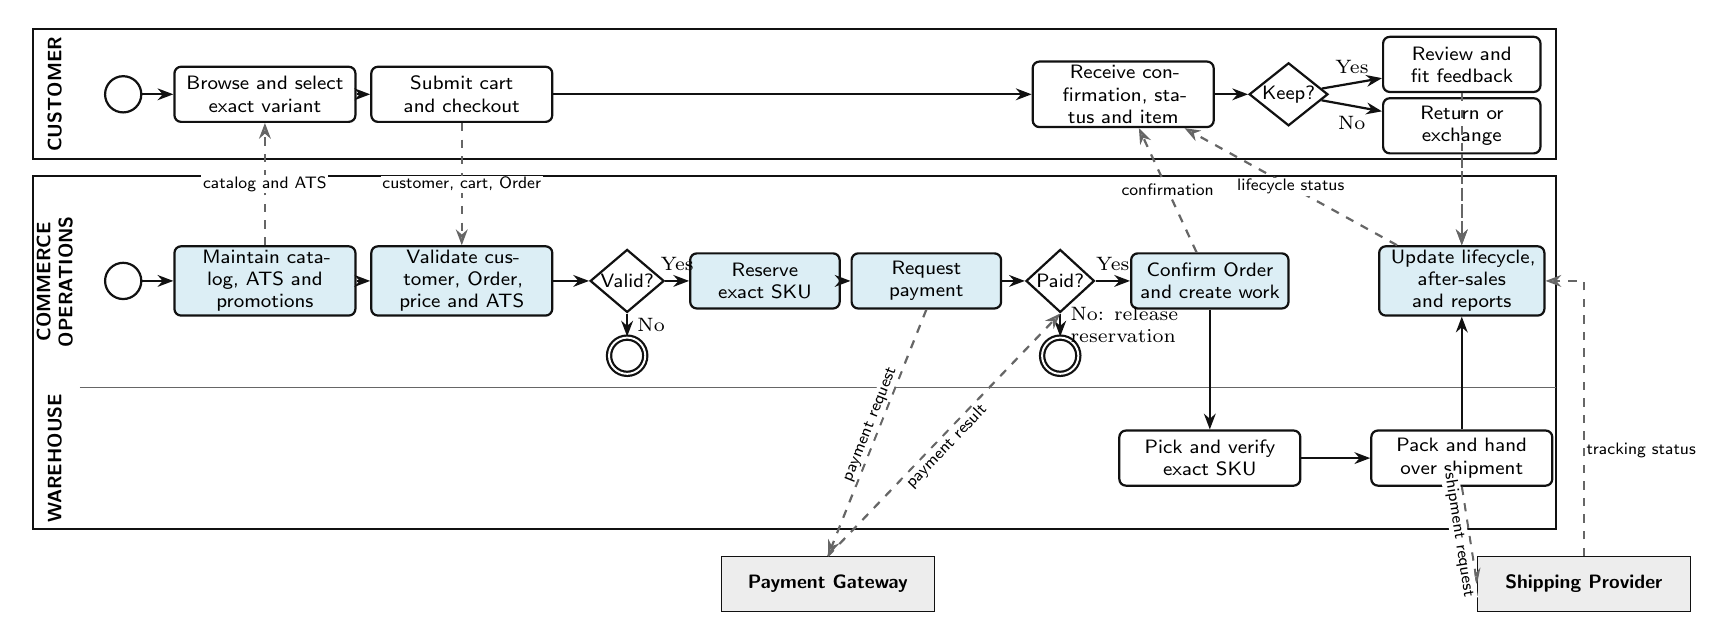
\begin{tikzpicture}[x=1cm,y=1cm]
  % Participant pools and ABC lanes
  \fill[LaneGray] (-.7,5.70) rectangle (18.65,7.35);
  \draw[pool] (-.7,5.70) rectangle (18.65,7.35);
  \node[rotate=90,font=\bfseries\sffamily\scriptsize] at (-.42,6.52) {CUSTOMER};
  \fill[LaneGray] (-.7,1.00) rectangle (18.65,2.80);
  \draw[pool] (-.7,1.00) rectangle (18.65,5.48);
  \draw[lane] (-.1,2.80)--(18.65,2.80);
  \node[rotate=90,font=\bfseries\sffamily\scriptsize,align=center] at (-.42,4.14) {COMMERCE\\OPERATIONS};
  \node[rotate=90,font=\bfseries\sffamily\scriptsize] at (-.42,1.90) {WAREHOUSE};

  % Customer pool
  \node[bpmnEvent] (cs) at (.45,6.52) {};
  \node[bpmnHuman] (browse) at (2.25,6.52) {Browse and select exact variant};
  \node[bpmnHuman] (checkout) at (4.75,6.52) {Submit cart and checkout};
  \node[bpmnHuman] (receive) at (13.15,6.52) {Receive confirmation, status and item};
  \node[bpmnGateway] (keep) at (15.25,6.52) {Keep?};
  \node[bpmnHuman,text width=19mm] (review) at (17.45,6.90) {Review and fit feedback};
  \node[bpmnHuman,text width=19mm] (return) at (17.45,6.12) {Return or exchange};
  \draw[sequence] (cs)--(browse); \draw[sequence] (browse)--(checkout);
  \draw[sequence] (checkout)--(receive); \draw[sequence] (receive)--(keep);
  \draw[sequence] (keep)--node[above,font=\scriptsize]{Yes}(review);
  \draw[sequence] (keep)--node[below,font=\scriptsize]{No}(return);

  % Commerce Operations lane
  \node[bpmnEvent] (as) at (.45,4.15) {};
  \node[bpmnTask] (catalog) at (2.25,4.15) {Maintain catalog, ATS and promotions};
  \node[bpmnTask] (validate) at (4.75,4.15) {Validate customer, Order, price and ATS};
  \node[bpmnGateway] (valid) at (6.85,4.15) {Valid?};
  \node[bpmnTask,text width=18mm] (reserve) at (8.60,4.15) {Reserve exact SKU};
  \node[bpmnTask,text width=18mm] (pay) at (10.65,4.15) {Request payment};
  \node[bpmnGateway] (auth) at (12.35,4.15) {Paid?};
  \node[bpmnTask,text width=19mm] (confirm) at (14.25,4.15) {Confirm Order and create work};
  \node[bpmnTask,text width=20mm] (status) at (17.45,4.15) {Update lifecycle, after-sales and reports};
  \node[bpmnEnd] (reject) at (6.85,3.20) {};
  \node[bpmnEnd] (failed) at (12.35,3.20) {};
  \draw[sequence] (as)--(catalog); \draw[sequence] (catalog)--(validate); \draw[sequence] (validate)--(valid);
  \draw[sequence] (valid)--node[above,font=\scriptsize]{Yes}(reserve); \draw[sequence] (reserve)--(pay);
  \draw[sequence] (pay)--(auth); \draw[sequence] (auth)--node[above,font=\scriptsize]{Yes}(confirm);
  \draw[sequence] (valid)--node[right,font=\scriptsize]{No}(reject);
  \draw[sequence] (auth)--node[right,font=\scriptsize,align=left]{No: release\\reservation}(failed);

  % Warehouse lane and end-to-end handoff
  \node[bpmnHuman] (pick) at (14.25,1.90) {Pick and verify exact SKU};
  \node[bpmnHuman] (pack) at (17.45,1.90) {Pack and hand over shipment};
  \draw[sequence] (confirm)--(pick); \draw[sequence] (pick)--(pack); \draw[sequence] (pack)--(status);

  % Message flows across participant boundaries
  \draw[message] (catalog)--node[flowlabel]{catalog and ATS}(browse);
  \draw[message] (checkout)--node[flowlabel]{customer, cart, Order}(validate);
  \draw[message] (confirm)--node[flowlabel]{confirmation}(receive);
  \draw[message] (status)--node[flowlabel]{lifecycle status}(receive);
  \draw[message] (review)--(status); \draw[message] (return)--(status);

  % External black-box pools
  \node[draw=Ink,fill=TableGray,font=\bfseries\sffamily\scriptsize,minimum width=27mm,minimum height=7mm] (gateway) at (9.40,.30) {Payment Gateway};
  \node[draw=Ink,fill=TableGray,font=\bfseries\sffamily\scriptsize,minimum width=27mm,minimum height=7mm] (carrier) at (19.00,.30) {Shipping Provider};
  \draw[message] (pay.south) -- node[flowlabel,above,sloped,pos=.48]{payment request} (gateway.north);
  \draw[message] (gateway.north) -- node[flowlabel,below,sloped,pos=.48]{payment result} (auth.south);
  \draw[message] (pack.south) -- node[flowlabel,below,sloped,pos=.48]{shipment request} (carrier.west);
  \draw[message] (carrier.north) -- node[flowlabel,right,pos=.50]{tracking status} (19.00,3.35) |- (status.east);
\end{tikzpicture}}
\caption{Core Diagram 2 --- High-Level Fashion Order-to-After-Sales Process (BPMN 2.0).}
\end{figure}
\fi
\begin{figure}[H]
\centering
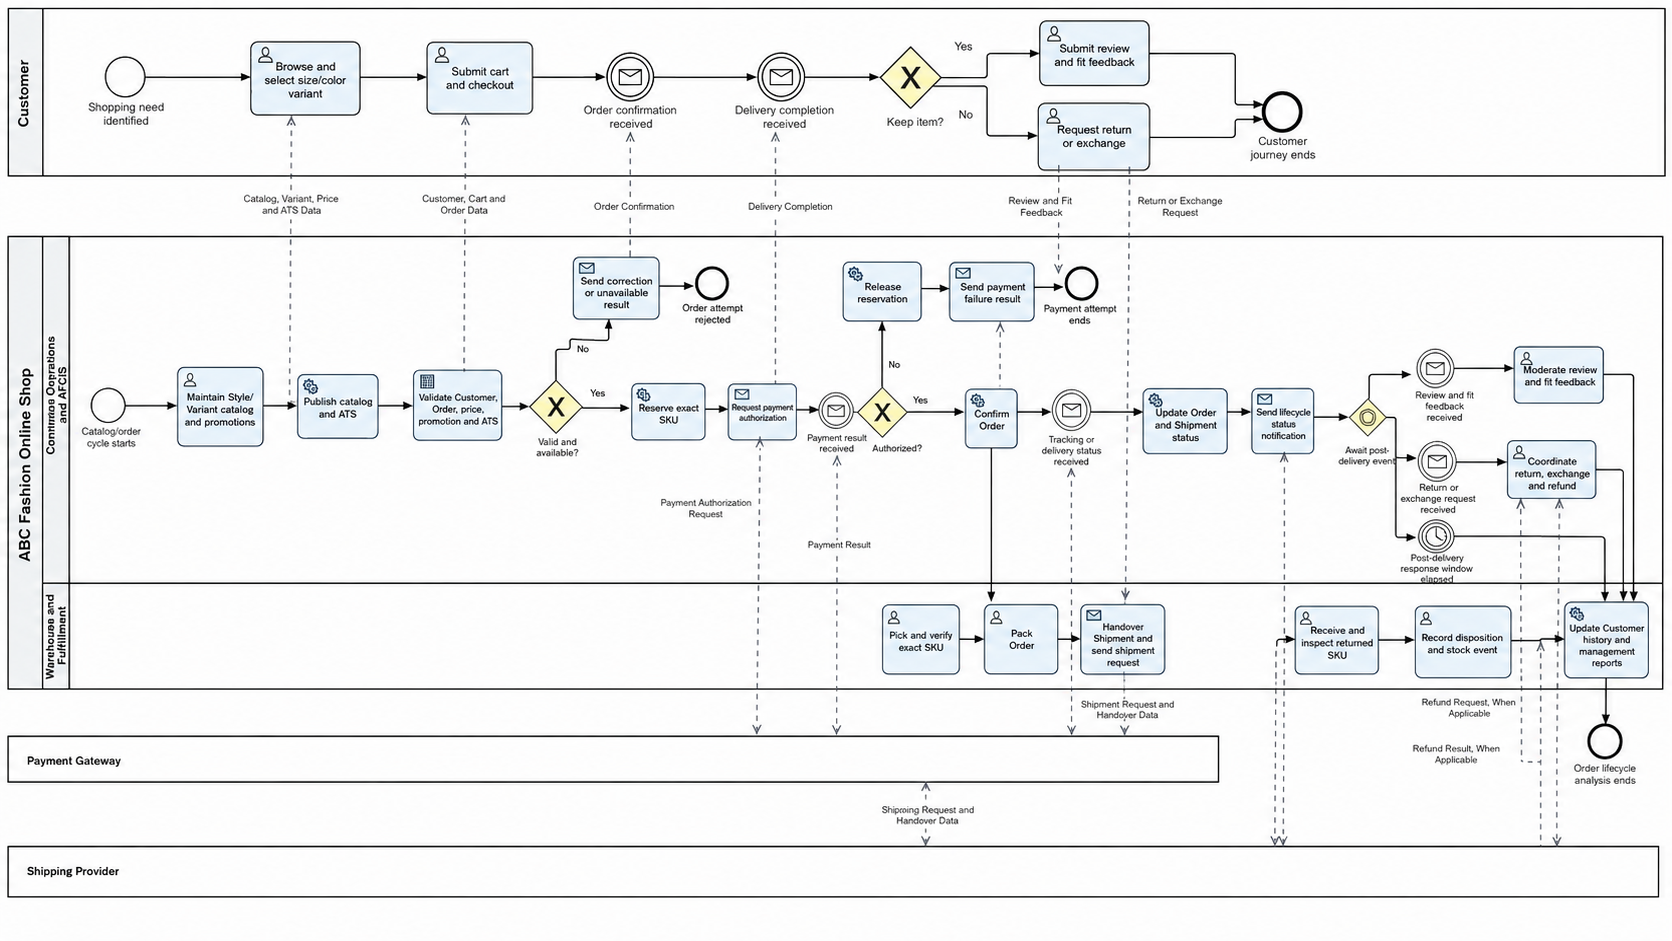
\includegraphics[width=0.98\textwidth]{bpmn_2.0.png}
\caption{Core Diagram 2 --- High-Level Fashion Order-to-After-Sales Process (BPMN 2.0).}
\label{fig:business-process}
\end{figure}

Solid Sequence Flows remain inside a pool; dashed Message Flows cross participant boundaries. External providers are black-box pools. Alternative validation, payment-failure, review, and return/exchange paths are shown without introducing detailed Use Cases.
\newpage

% ============================== PAGE 5 ==============================
\section{Information Analysis}
\subsection{Information Produced}
Approved catalog/variant records, carts, Orders and line snapshots, reservations/movements, payment/refund requests, confirmations, pick/pack work, shipment requests/status, notifications, after-sales cases, reviews, audit events and reports.

\subsection{Information Consumed}
Supplier product facts; customer identity, contact, address and consent; searches, carts and checkout selections; size and fit data; price and promotion rules; ATS; gateway results; warehouse events; carrier milestones; return reasons; and report parameters.

\subsection{Information Stored}
AFCIS stores controlled Product Style/Variant masters; media/size-fit metadata; prices/promotions; customer data; carts as policy permits; Orders and immutable line snapshots; SKU inventory/reservations/movements; gateway references/statuses; fulfillment, shipment and notification events; returns/exchanges/refunds; reviews and audit history. Raw card numbers/CVV, carrier routing, supplier manufacturing data and the accounting ledger remain outside.

\subsection{Information Catalogue}
\begin{tabularx}{\textwidth}{L{9mm}L{35mm}L{29mm}Y L{20mm}}
\rowcolor{TableGray}\textbf{ID} & \textbf{Information} & \textbf{Source} & \textbf{Purpose / principal users} & \textbf{Lifecycle}\\
I-01--03 & Style, Variant/SKU, media and size/fit/care & Merchandiser; supplier facts & Exact product discovery, selection, stock and fulfillment & P/C/S/X\\
I-04 & Price and promotion rule/result & Marketing / Manager & Consistent presentation, checkout and reporting & P/C/S/X\\
I-05 & Customer, address, preference and consent & Customer / authorized staff & Checkout, service and controlled communication & P/C/S/X\\
I-06--07 & Cart, checkout, Order and line snapshot & Customer / AFCIS & Commercial commitment and coordination & P/C/S/X\\
I-08 & Inventory balance, reservation, movement, ATS & Warehouse / AFCIS & Variant-level availability and traceability & P/C/S\\
I-09 & Payment/refund request, reference and status & AFCIS / Gateway & Coordinate and reconcile without raw card data & P/C/S/X\\
I-10--12 & Fulfillment, shipment/tracking, notification & Warehouse / providers & Direct work and explain lifecycle status & P/C/S/X\\
I-13 & Cancellation, return, exchange and refund case & Customer, staff, Gateway & Control reverse logistics, replacement and money & P/C/S/X\\
I-14 & Review and fit feedback & Customer / moderator & Product insight and approved social proof & P/C/S/X\\
I-15 & Supplier, receipt and discrepancy & Supplier / Warehouse & Replenishment and stock receipt administration & P/C/S\\
I-16--17 & KPI/report and status/audit event & AFCIS / actors & Decisions, exceptions, reproducibility, accountability & P/C/S/X\\
\end{tabularx}
\footnotesize P = produced/updated; C = consumed; S = stored; X = exchanged across the AFCIS boundary.

\normalsize\textbf{Preliminary information-quality rules}
\begin{enumerate}
\item Every active Product Variant belongs to one Product Style and has a unique SKU; the Style itself is not stocked or ordered.
\item Published Variants contain applicable size/system, color, material/pattern/fit, approved media, price, state and availability source.
\item Every stock event references exact SKU, location, signed quantity, event type/time, actor/source and originating reference.
\item An Order Line preserves the committed SKU, description, attributes, price, discount and quantity after catalog changes.
\item Order, Payment, Shipment, Return, Exchange and Refund use controlled, timestamped status transitions.
\item Payment data is minimized; raw PAN and CVV/CVC are excluded. Customer/consent changes are attributable.
\item Reports state period, included statuses and refresh/cut-off time so results are reproducible.
\end{enumerate}

All major activities have identifiable inputs and outputs, and the Product Variant remains the cart, stock, order-line, pick, return and exchange unit throughout.
\newpage

% ============================== PAGE 6 ==============================
\section{Current Problems}
\subsection{Problem Identification}
\begin{tabularx}{\textwidth}{L{9mm}Y L{27mm}L{25mm}}
\rowcolor{TableGray}\textbf{ID} & \textbf{Significant problem} & \textbf{Affected information} & \textbf{Evidence}\\
P-01 & Inconsistent product information can make Style, size/color Variant, media, price and publication disagree. & I-01--04 & Case fact; fashion extension\\
P-02 & Outdated inventory may not represent ATS for the exact size/color SKU. & I-02, I-08 & Case fact; variant extension\\
P-03 & Manual order steps and disconnected handoffs cause delay and re-keying risk. & I-06--11 & Case fact\\
P-04 & Customers/staff cannot always obtain one accurate, timely lifecycle status. & I-07, I-09, I-11--13, I-17 & Case fact; after-sales extension\\
P-05 & Customer data in different places creates duplicate/inconsistent identity, address, consent and history. & I-05, I-07, I-12--13 & Case fact\\
P-06 & Manual reports and limited real-time information delay and weaken management decisions. & I-07--09, I-11, I-13, I-16 & Case fact\\
P-07 & Return/exchange, inspection, restock and refund may lack one traceable lifecycle. & I-02, I-07--09, I-13, I-17 & Domain hypothesis\\
P-08 & Promotion rules may be inconsistent across catalog, cart, order, service and reports. & I-04, I-06--07, I-16--17 & Hypothesis\\
\end{tabularx}

\subsection{Problem Causes}
Candidate causes are: no governed Style/Variant master or clear ownership (C-01); delayed/manual or wrong-granularity stock events (C-02); separate order/payment/stock/shipping/after-sales queues (C-03); fragmented customer capture (C-04); inconsistent status vocabulary/ownership (C-05); manual report consolidation (C-06); and uncontrolled promotion eligibility/effective-date/stacking rules (C-07). These require catalog audits, process walkthroughs, cycle counts, source inventories and status/rule workshops.

\subsection{Problem Consequences}
The combined effects are inaccurate promise or cancellation; overselling, underselling and wrong-variant picks; staff re-keying and reconciliation; delayed or conflicting customer status; duplicate customer and consent risk; slower assortment, replenishment and promotion decisions; and broken financial and operational traceability.

\subsection{Problem Tree}
\iffalse
\begin{figure}[!h]
\centering
\resizebox{0.98\textwidth}{!}{%
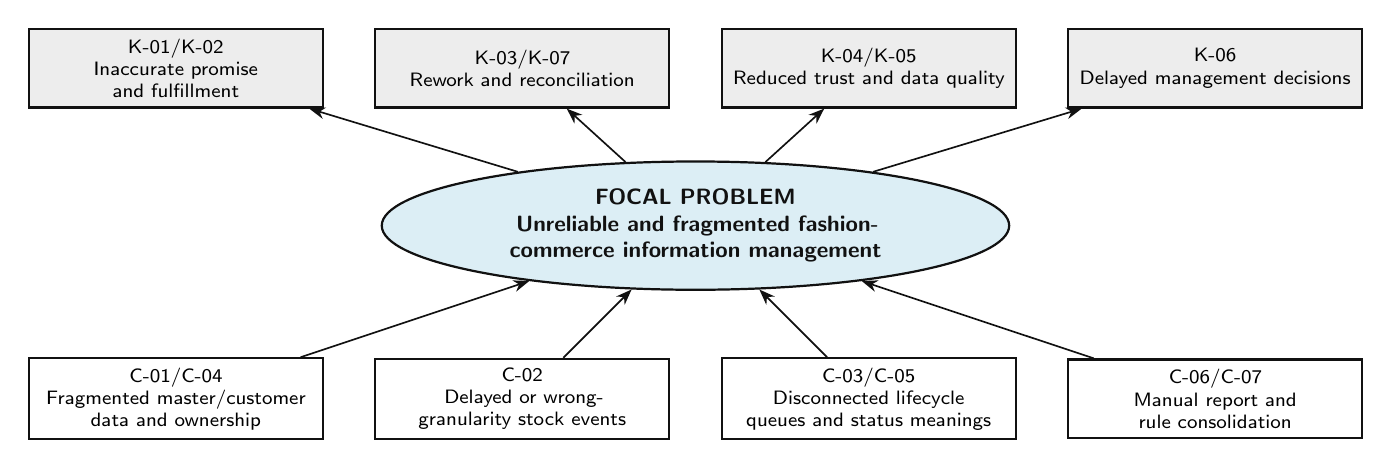
\begin{tikzpicture}[x=1cm,y=1cm]
  \node[effect] (k1) at (-6.6,3.0) {K-01/K-02\\Inaccurate promise and fulfillment};
  \node[effect] (k2) at (-2.2,3.0) {K-03/K-07\\Rework and reconciliation};
  \node[effect] (k3) at (2.2,3.0) {K-04/K-05\\Reduced trust and data quality};
  \node[effect] (k4) at (6.6,3.0) {K-06\\Delayed management decisions};
  \node[focal] (p) at (0,1.0) {FOCAL PROBLEM\\Unreliable and fragmented fashion-commerce information management};
  \node[cause] (c1) at (-6.6,-1.2) {C-01/C-04\\Fragmented master/customer data and ownership};
  \node[cause] (c2) at (-2.2,-1.2) {C-02\\Delayed or wrong-granularity stock events};
  \node[cause] (c3) at (2.2,-1.2) {C-03/C-05\\Disconnected lifecycle queues and status meanings};
  \node[cause] (c4) at (6.6,-1.2) {C-06/C-07\\Manual report and rule consolidation};
  \foreach \c in {c1,c2,c3,c4}{\draw[causal] (\c)--(p);}
  \foreach \k in {k1,k2,k3,k4}{\draw[causal] (p)--(\k);}
\end{tikzpicture}}
\caption*{\textbf{PT-1.} Mandatory supporting Problem Tree. Causes appear below the focal problem and consequences above it; arrows mean ``contributes to.''}
\end{figure}
\fi
\begin{figure}[H]
\centering
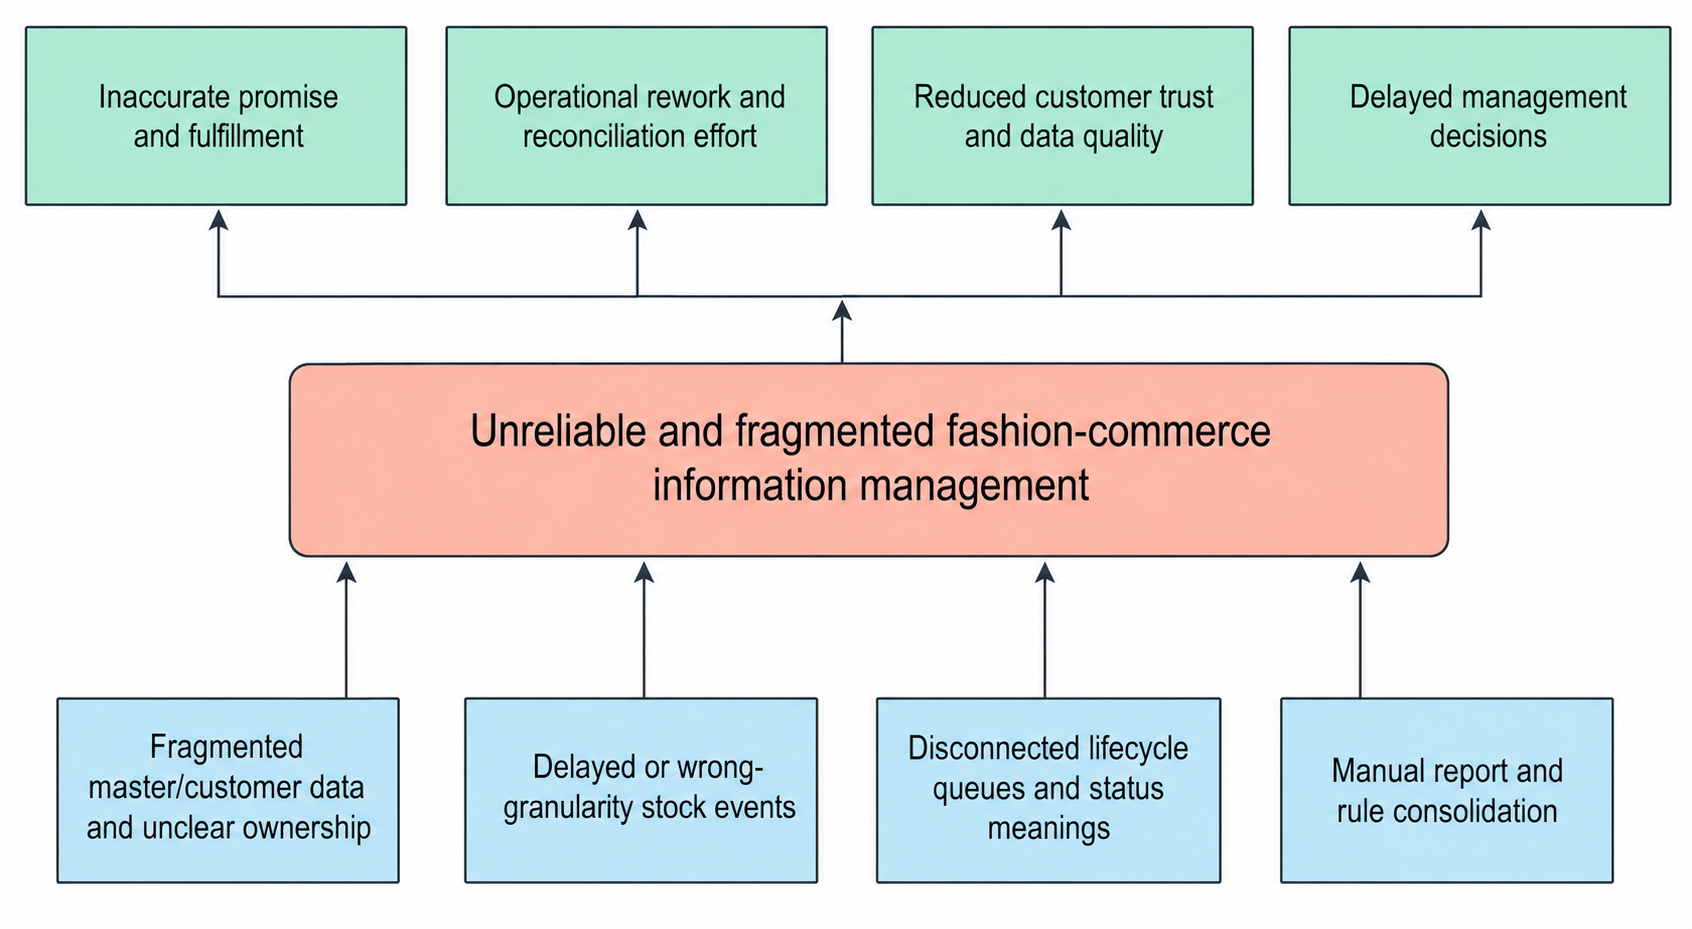
\includegraphics[width=0.88\textwidth]{problem_tree.png}
\caption*{\textbf{PT-1.} Mandatory supporting Problem Tree. Causes appear below the focal problem and consequences above it; arrows mean ``contributes to.''}
\label{fig:problem-tree}
\end{figure}

P-01--P-04 are investigated first because they determine whether the exact Variant can be promised, paid, fulfilled and explained. P-05--P-06 share the same source-of-truth need; P-07--P-08 remain in preliminary scope only if early validation confirms them.
\newpage

% ============================== PAGE 7 ==============================
\section{Proposed Information System}
\subsection{System Purpose}
The proposed \keyterm{ABC Fashion Commerce Information System (AFCIS)} provides one controlled operational backbone for Style/Variant, customer, price/promotion, Order, payment-reference, inventory, fulfillment, shipment, after-sales, review and reporting information. It is justified by P-01--P-06, not by a solution-first desire to build a website.

\subsection{System Scope}
\begin{tabularx}{\textwidth}{L{12mm}Y L{36mm}}
\rowcolor{TableGray}\textbf{ID} & \textbf{Capability inside AFCIS} & \textbf{Problems addressed}\\
S-01 & Controlled category, Style/Variant, media, size/fit/care and publication management & P-01, P-02\\
S-02 & Customer profile, address, consent and authorized service-history management & P-04, P-05\\
S-03 & Variant-aware browsing, cart, checkout, price/promotion and ATS validation & P-01, P-02, P-08\\
S-04 & Order snapshot/status, reservation, cancellation, payment/refund orchestration and confirmation & P-02--04, P-07--08\\
S-05 & SKU/location stock, reservation, movement, pick/pack, adjustment and return disposition & P-01--03, P-07\\
S-06 & Shipment request/tracking integration, lifecycle timeline and notification orchestration & P-03, P-04\\
S-07 & Return, exchange, inspection, replacement and refund-case coordination & P-04, P-07\\
S-08 & Eligible review, moderation state and fit-feedback capture & Supports business objectives\\
S-09 & Operational dashboards/reports, exceptions, reconciliation and audit history & P-02--04, P-06, P-08\\
S-10 & Roles, reference values, status definitions and workflow/policy administration & P-01, P-04--06, P-08\\
\end{tabularx}

Scope principles are one operational source of truth, exact-Variant traceability, event-linked lifecycle status, and external specialization remaining external. The scope defines information responsibility, not screens, tables, APIs, hosting or code.

\subsection{System Boundary}
\begin{tabularx}{\textwidth}{L{23mm}Y Y}
\rowcolor{TableGray}\textbf{Area} & \textbf{Inside AFCIS} & \textbf{Outside / boundary rationale}\\
Customer and product & Catalog, account, cart, checkout, Order, status, content, price/promotion & Customer device/decisions; supplier manufacturing and creative tools\\
Payment & Request orchestration, amount/reference/status and reconciliation & Gateway captures credentials and executes authorization/capture/refund\\
Inventory and warehouse & Stock records, ATS, reservations, work queues and physical-event capture & Merchandise, shelving/equipment and human physical execution\\
Shipping and notification & Shipment/message requests, tracking/status, customer timeline and logs & Carrier routing/transport and provider delivery infrastructure\\
Service and reporting & Consolidated timeline, cases, KPIs, exceptions and governed exports & Human conversations/discretion; general ledger, tax, payroll and enterprise BI\\
Procurement & Supplier master, expected receipt, discrepancy and replenishment note & Supplier portal, sourcing, contracts and full purchase-to-pay\\
\end{tabularx}

\textbf{Explicit exclusions:} detailed UML Use Cases and requirements; ERD/database/component/deployment/API/UI design and code; marketplace sellers/commissions; physical POS; payment credentials and gateway internals; carrier fleet/routing; supplier manufacturing/procurement automation; general ledger/tax/payroll/HR; and advanced AI recommendation, dynamic pricing or forecasting.

\textbf{Dependencies and controls:} provider contracts/interfaces and exception rules; catalog/customer/stock/order profiling before migration; approved publication, promotion, reservation, cancellation, return/exchange/refund and status policies; role-based handling of personal/payment-restricted information; and timely staff capture of physical events.

\colorbox{TableGray}{\parbox{\dimexpr\textwidth-2\fboxsep}{\footnotesize
\textbf{Boundary rationale.} AFCIS records and explains requests/results but does not perform payment processing, parcel transport or message delivery. Supplier is a business stakeholder but not a direct system interface in the initial boundary; authorized staff record relevant receipt/replenishment inputs.}}
\newpage

% ============================== PAGE 8 ==============================
\subsection{Context Diagram}
Figure 3 uses one black-box DFD process, seven external entities, sixteen directed noun-phrase information flows and no data store or internal subprocess.

\iffalse
\begin{figure}[!h]
\centering
\resizebox{0.98\textwidth}{!}{%
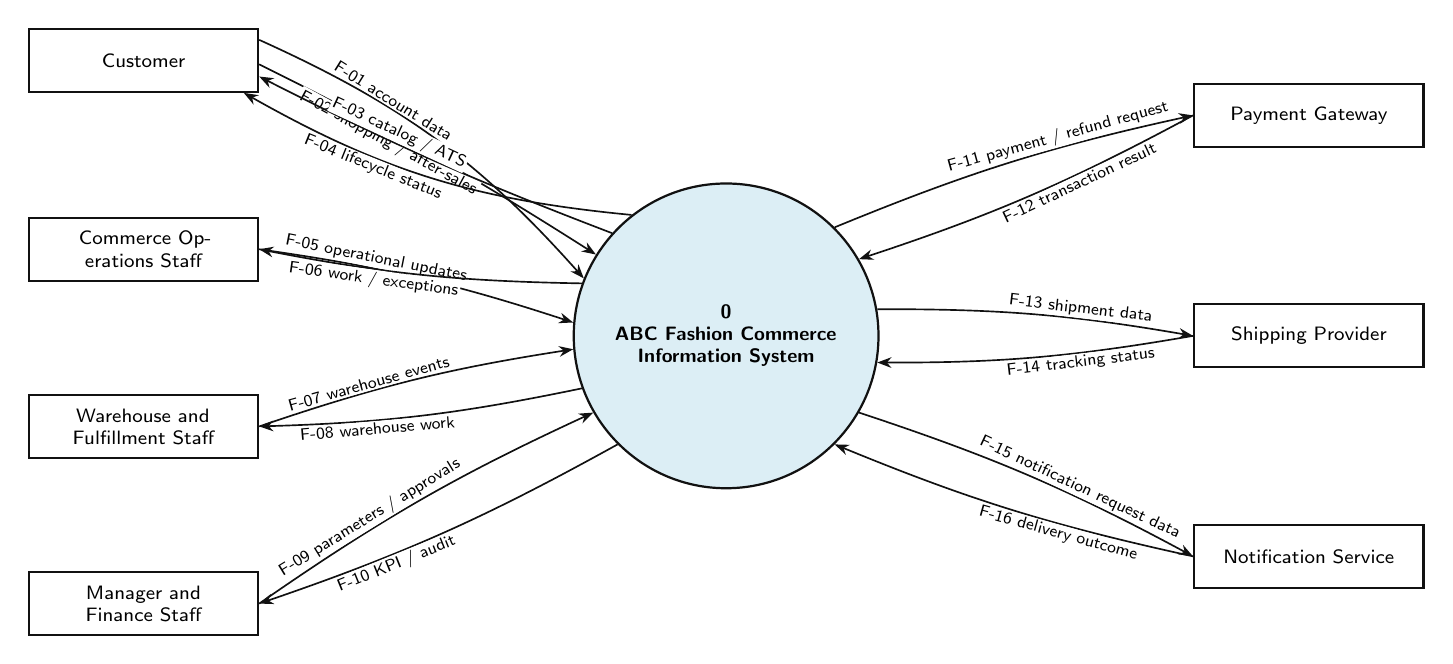
\begin{tikzpicture}[x=1cm,y=1cm]
  \node[dfdProcess] (sys) at (0,0) {0\\ABC Fashion Commerce\\Information System};
  \node[dfdEntity] (c) at (-7.4,3.50) {Customer};
  \node[dfdEntity] (o) at (-7.4,1.1) {Commerce Operations Staff};
  \node[dfdEntity] (w) at (-7.4,-1.15) {Warehouse and Fulfillment Staff};
  \node[dfdEntity] (m) at (-7.4,-3.4) {Manager and Finance Staff};
  \node[dfdEntity] (p) at (7.4,2.8) {Payment Gateway};
  \node[dfdEntity] (s) at (7.4,0) {Shipping Provider};
  \node[dfdEntity] (n) at (7.4,-2.8) {Notification Service};
  % Customer has four distinct one-way flows; other entities have one pair each.
  \draw[dataflow] (c.10) to[bend left=12] node[flowlabel,above,sloped,pos=.35]{F-01 account data} (sys.158);
  \draw[dataflow] (c.-2) to[bend left=3] node[flowlabel,below,sloped,pos=.38]{F-02 shopping / after-sales} (sys.148);
  \draw[dataflow] (sys.138) to[bend left=3] node[flowlabel,above,sloped,pos=.62]{F-03 catalog / ATS} (c.-8);
  \draw[dataflow] (sys.128) to[bend left=12] node[flowlabel,below,sloped,pos=.65]{F-04 lifecycle status} (c.-18);
  \draw[dataflow] (o.east) to[bend left=5] node[flowlabel,above,sloped,pos=.35]{F-05 operational updates} (sys.175);
  \draw[dataflow] (sys.160) to[bend left=5] node[flowlabel,below,sloped,pos=.65]{F-06 work / exceptions} (o.east);
  \draw[dataflow] (w.east) to[bend left=5] node[flowlabel,above,sloped,pos=.35]{F-07 warehouse events} (sys.185);
  \draw[dataflow] (sys.200) to[bend left=5] node[flowlabel,below,sloped,pos=.65]{F-08 warehouse work} (w.east);
  \draw[dataflow] (m.east) to[bend left=5] node[flowlabel,above,sloped,pos=.35]{F-09 parameters / approvals} (sys.210);
  \draw[dataflow] (sys.225) to[bend left=5] node[flowlabel,below,sloped,pos=.65]{F-10 KPI / audit} (m.east);
  % right-side paired flows
  \draw[dataflow] (sys.45) to[bend left=5] node[flowlabel,above,sloped,pos=.65]{F-11 payment / refund request} (p.west);
  \draw[dataflow] (p.west) to[bend left=5] node[flowlabel,below,sloped,pos=.35]{F-12 transaction result} (sys.30);
  \draw[dataflow] (sys.10) to[bend left=5] node[flowlabel,above,sloped,pos=.65]{F-13 shipment data} (s.west);
  \draw[dataflow] (s.west) to[bend left=5] node[flowlabel,below,sloped,pos=.35]{F-14 tracking status} (sys.-10);
  \draw[dataflow] (sys.-30) to[bend left=5] node[flowlabel,above,sloped,pos=.65]{F-15 notification request data} (n.west);
  \draw[dataflow] (n.west) to[bend left=5] node[flowlabel,below,sloped,pos=.35]{F-16 delivery outcome} (sys.-45);
\end{tikzpicture}}
\caption{Core Diagram 3 --- AFCIS System Context Diagram (Yourdon--DeMarco DFD convention).}
\end{figure}
\fi
\begin{figure}[H]
\centering
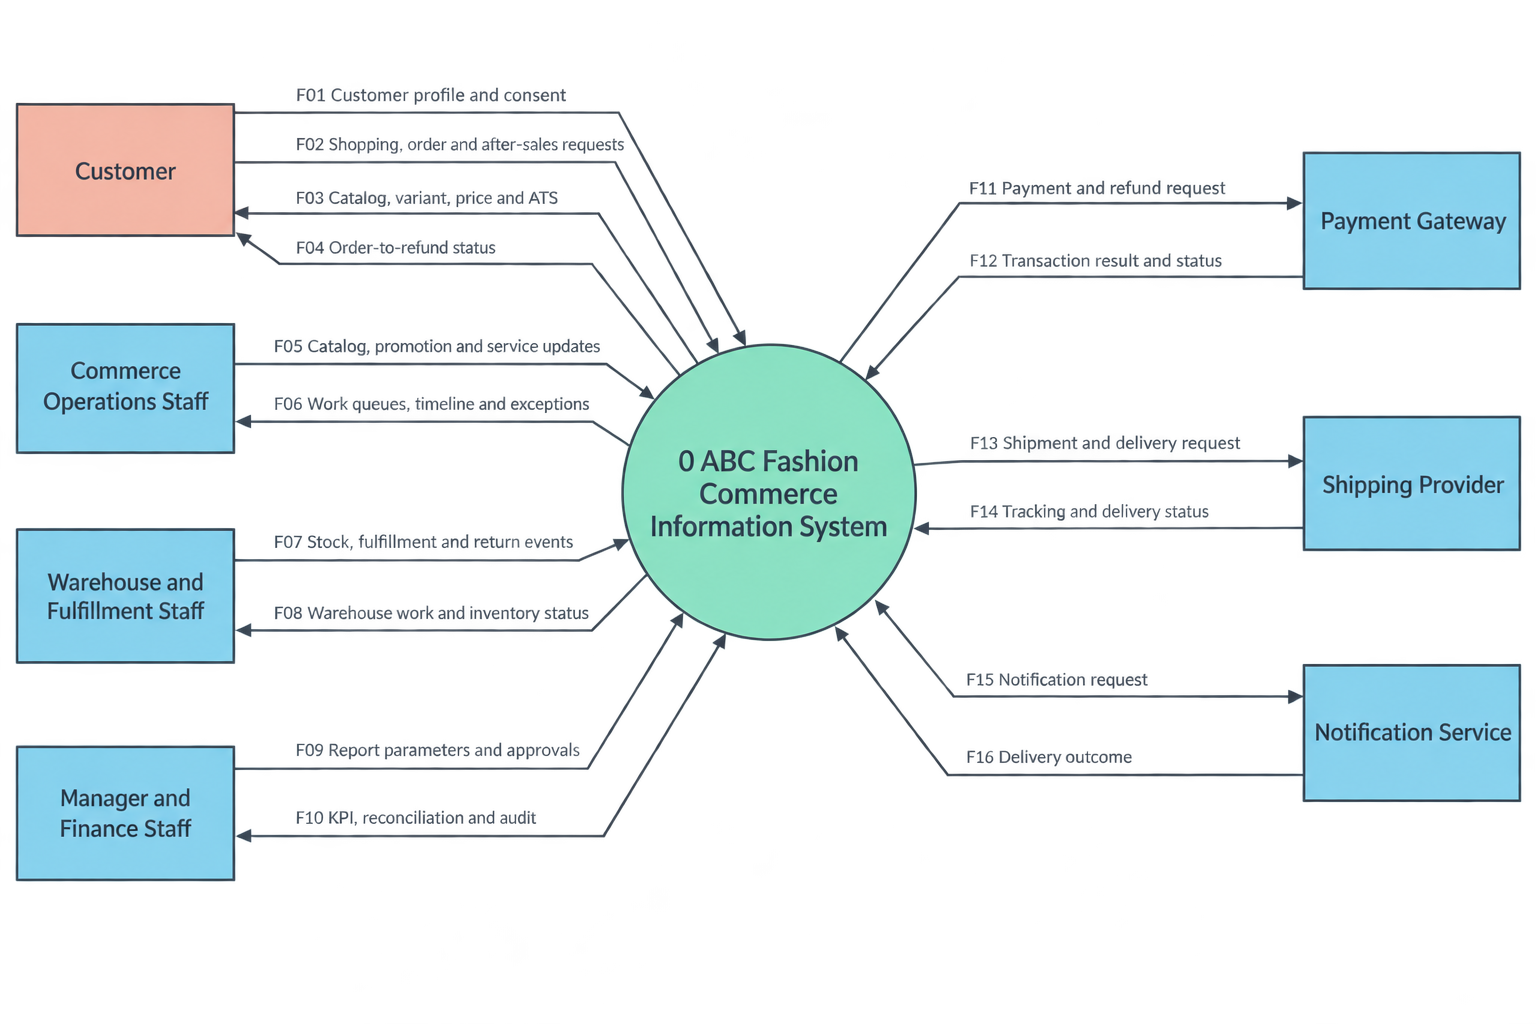
\includegraphics[width=0.98\textwidth]{context_diagram.png}
\caption{Core Diagram 3 --- AFCIS System Context Diagram (Yourdon--DeMarco DFD convention).}
\label{fig:context-diagram}
\end{figure}

\subsection{Information Flows}
\begin{tabularx}{\textwidth}{L{13mm}L{32mm}L{32mm}Y}
\rowcolor{TableGray}\textbf{Flow} & \textbf{Source} & \textbf{Destination} & \textbf{Information crossing the boundary}\\
F-01--02 & Customer & AFCIS & Account/contact/consent; search, cart, checkout, Order, review and after-sales requests\\
F-03--04 & AFCIS & Customer & Catalog/Variant/size-fit/price/ATS; checkout and full lifecycle status\\
F-05--06 & Operations Staff / AFCIS & AFCIS / Operations Staff & Catalog/promotion/service/admin updates; work, timeline, quality and exceptions\\
F-07--08 & Warehouse Staff / AFCIS & AFCIS / Warehouse Staff & Receipt/count/pick/pack/return events; exact-SKU work and inventory status\\
F-09--10 & Manager/Finance / AFCIS & AFCIS / Manager/Finance & Parameters/targets/approvals; KPI, reconciliation and audit information\\
F-11--12 & AFCIS / Gateway & Gateway / AFCIS & Payment/capture/refund requests; transaction references and results\\
F-13--14 & AFCIS / Carrier & Carrier / AFCIS & Shipment/package/recipient data; tracking, milestone, delivery and exception status\\
F-15--16 & AFCIS / Notification Service & Service / AFCIS & Destination/content/template request; acceptance, delivery or failure outcome\\
\end{tabularx}

Every context entity has at least one named incoming and outgoing flow. Payment, shipping and notification providers remain external. The DFD contains no entity-to-entity flow, database, UI or implementation component.
\newpage

% ============================== PAGE 9 ==============================
\subsection{System Objectives}
\begin{tabularx}{\textwidth}{L{10mm}Y L{39mm}}
\rowcolor{TableGray}\textbf{ID} & \textbf{Preliminary objective} & \textbf{Candidate measure / target}\\
O-01 & One governed Style/Variant catalog with complete fashion attributes and controlled publication. & 100\% of published Variants pass mandatory-field and unique-SKU validation.\\
O-02 & Timely, traceable SKU-level inventory, reservations, movements and ATS. & At least 99\% physical-to-record accuracy; accepted event visible within 60 seconds.\\
O-03 & Coordinate routine Orders from checkout through payment, stock, fulfillment and shipment without re-keying. & At least 90\% of routine paid Orders enter warehouse work without manual re-entry.\\
O-04 & One timely, explainable lifecycle status for customers and staff with proactive notifications. & At least 95\% of accepted status events visible within five minutes.\\
O-05 & Traceable cancellation, return, size/color exchange, inspection, restock, replacement and refund. & 100\% of approved cases retain linked Order Line/SKU, decision, disposition and financial status.\\
O-06 & Controlled customer data and secure external payment coordination without raw card credentials. & 100\% use gateway references; zero raw PAN/CVV stored; profile duplicates before target-setting.\\
O-07 & Timely, reproducible operational reports and exception views. & Agreed dashboards refresh within 15 minutes; standard reports need no manual source consolidation.\\
\end{tabularx}

Targets are provisional until ABC measures the current baseline and approves definitions in Assignment 02. Together, O-01--O-07 trace to every case-established problem P-01--P-06; O-02/O-05 and O-01/O-07 also cover P-07/P-08 if those hypotheses are confirmed.

\section{Conclusion}
ABC does not primarily need ``a website.'' It needs to solve a more fundamental information problem: fragmented and unreliable Style/Variant, inventory, customer, Order, external-service status, after-sales and reporting information prevents the business from promising, fulfilling, explaining and learning from the lifecycle of the exact fashion Product Variant.

AFCIS responds with a bounded, traceable information-system proposal. It governs the Style/Variant distinction and coordinates catalog, customer, cart, Order, payment-reference, stock, fulfillment, shipment, return/exchange/refund, review and reporting information. Payment execution, physical transport, message delivery, supplier systems and accounting stay outside with named crossings. Before Assignment 02, ABC should validate candidate causes and P-07/P-08, baseline objective measures, confirm policies/status vocabularies, and verify provider interfaces. Only then should stakeholders, problems, activities and information flows become formal actors, requirements and Use Cases.

\section{References}
\begin{enumerate}[label={[R\arabic*]},leftmargin=8mm,itemsep=.3pt]
\footnotesize
\item Tran, D. Q. (2026). \emph{Information System Analysis and Design --- Assignment 01: E-Commerce Information System Investigation}. Department of Information Technology, PTIT.
\item GS1 (2024). \emph{How many GS1 GTINs do I need when I have a product with many sizes and colours?}
\item Google Merchant Center. \emph{Product data specification} (variant-group, color, size, material and pattern guidance).
\item Baymard Institute. \emph{Apparel \& Accessories Ecommerce UX Research}.
\item PCI Security Standards Council. \emph{Merchant Resources --- What is PCI DSS?}
\item Object Management Group. \emph{Business Process Model and Notation (BPMN), Version 2.0.2}.
\item Visual Paradigm. \emph{Mind Mapping, BPMN Pool/Lane, System Context Diagram and Data Flow Diagram guidance}.
\end{enumerate}

\vfill
\begin{center}
\colorbox{TableGray}{\parbox{0.93\textwidth}{\centering\footnotesize
\textbf{Submission check:} three numbered core diagrams + supporting PT-1; no UML Use Case Diagram; consistent Product Style/Product Variant terminology; seven objectives; nine total PDF pages. Replace identity placeholders before submission.}}
\end{center}

\end{document}
